% !TeX spellcheck = en_US

\chapter{Software Design}
This chapter evaluates the possibility to use microservices for the WebUI components. It also describes the way, the user takes through the system. Finally the REST APIs consumed by the WebUI are described.



\section{Microservices for the WebUI}
The MARS Websuite has been transfered into a mircroservice architecture. Backend services communicate via REST instead of local system calls. While this works very well for the backend, frontend components behave much different.\\
The code of a backend service is executed in an environment defined by the provider of the application, while the frontend is delivered to the user and executed by his browser.


\subsection{Constraints}
The bearing mentioned above, brings certain restrictions which are for technical and security reason. The following constraints have to be considered.

\subsubsection{Cross-origin issue}
Cross-origin requests are API calls to an IP or port other than the one, that provided the original webpage. These kind of requests can reveal confidential information stored in the session or a cookie inside the browser to a third party.\\
Therefore modern browsers implement the \textit{same-origin policy} as specified in the \textit{RFC 6454 -- The Web Origin Concept} by \cite{barth2011web}, which blocks cross-origin requests.\\
Write access to cross-origin locations and certain tags are excluded from the restrictions, among them are \textit{<a>} \textit{<img>}, \textit{<video>}, \textit{<iframe>} and \textit{@font-face}. While not reccomended, it is also possible to deactivate the strict origin policy.

\subsubsection{Only one initial URL}
The user opens a website by typing an URL to the address-bar of his browser. This implies, that one endpoint needs to deliver the whole side. This page has to either load other parts dynamically, or has to aggregate the content of the other frontend microservices in the backend, before it is delivered to the browser.

\subsubsection{tightly coupled}
As mentioned in Section \ref{sec:angularjs}, the Websuite consists of an AngularJS single-page application. This implies, that it is indeed a single page, that uses routing to redirect from different pages. That being said, it is not possible to fetch single pages from another service during runtime.

\subsection{Solutions}
The cross-origin issue is quite common for any site that has more than one backend to communicate with. The solution is, to deliver the whole page and all the consumed REST endpoints over a reverse proxy. The Websuite does this via Zuul.\\
The harder part is to split up the frontend. To do this, there are a few options.

\subsubsection{Only static content}
Each service renders its static html. it is then combined and linked. This Approach is very easy, but is not suited for a dynamic web 2.0 application.

\subsubsection{Fullstack services}
Each frontend service has its own backend.

\subsubsection{Web Components}
% https://en.wikipedia.org/wiki/Web_Components


\section{Work-flow}
% Way of the user through the system

\begin{figure}[H]
	\centering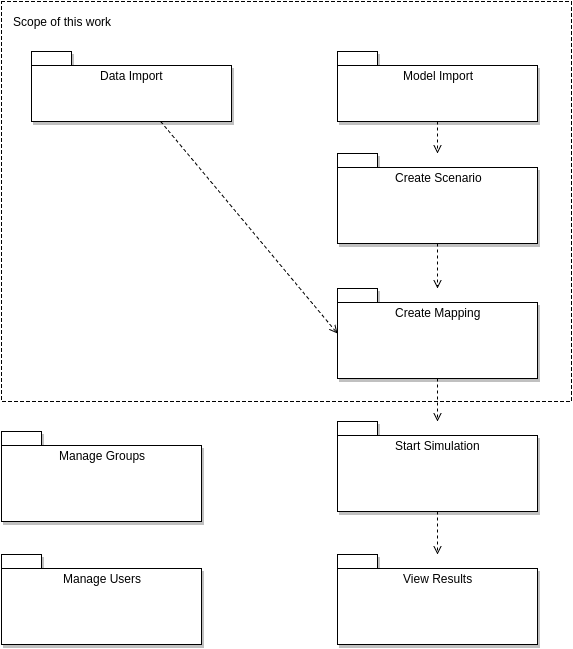
\includegraphics[width=.7\textwidth]{res/Dependency-workflow}
	\caption{Dependency work-flow}
	\label{fig:dependency-workflow}
\end{figure}



\section{Interface Description}
% rest Aufrufe